\documentclass[9pt]{article}

%%%%%%%%%%%%%%%%
%%% Packages %%%
%%%%%%%%%%%%%%%%

\usepackage[utf8]{inputenc}
\usepackage[english]{babel}
\usepackage{graphicx}
\usepackage{epstopdf}
\usepackage{amsmath,amssymb,amsbsy,amsthm,color}
\usepackage[paperwidth=18cm,paperheight=29.7cm,hmargin=2cm,vmargin=3cm]{geometry}

\usepackage[square,numbers]{natbib}

\graphicspath{{figures/}}


\begin{document}

\bibliographystyle{natbib}
	
\title{The Method of Lagrangian Descriptors}

\date{}
	
% \author{V. J. Garc\'{i}a-Garrido}
	
\maketitle

One of the biggest challenges of Dynamical Systems Theory or Nonlinear Dynamics is the development of mathematical techniques that provide us with the capability of exploring the geometrical template of structures that governs transport in phase space. Since the early 1900, the pioneering work carried out by Henri Poincar\'e on the three body problem of Celestial Mechanics \cite{hp1890}, the idea of pursuing a qualitative description of the solutions of differential equations has had a profound impact on the analysis of nonlinear phenomena that occurs in Nature. Indeed, this powerful approach has now been widely embraced by the scientific community and its essence has been nicely captured by Vladimir Arnold's statement that the complete understanding of nonlinear dynamics boils down to the geometrical analysis of phase space. 

In this chapter we present the details of a mathematical tool whose potential has shown to bring us one step closer to fulfilling the long-soght dream envisioned by Poincar\'e. The method is known in the literature as Lagrangian descriptors (LDs), which is a trajectory-based scalar diagnostic with the capability of revealing the geometrical template of phase space structures that characterizes qualitatively distinct dynamical behavior. This technique was introduced a decade ago in \cite{madrid2009} to analyze Lagrangian transport and mixing in Geophysical flows \cite{mendoza2010}, and was originally defined by means of computing the arclength of the trajectories of initial conditions as they evolve forward and backward in time \cite{mancho2013lagrangian}. The approach provided by Lagrangian descriptors to unveil the skeleton of dynamical processes has found a myriad of applications in different scientific areas. For instance, in the context of Oceanography it has been used to plan transoceanic autonomous underwater vehicle missions by taking advantage of the underlying dynamical structure of ocean currents \cite{ramos2018}. Recently, this tool has also received recognition in the field of Chemistry, in particular in Transition State Theory \cite{craven2015lagrangian,craven2016deconstructing,craven2017lagrangian}, where the computation of chemical reaction rates relies on the knowledge of the phase space structures that separate reactants from products. These high-dimensional structures characterizing reaction dynamics are typically related to Normally Hyperbolic Invariant Manifolds (NHIMs) and their stable and unstable manifolds that occur in Hamiltonian systems.

\begin{figure}[htbp]
	\begin{center}
		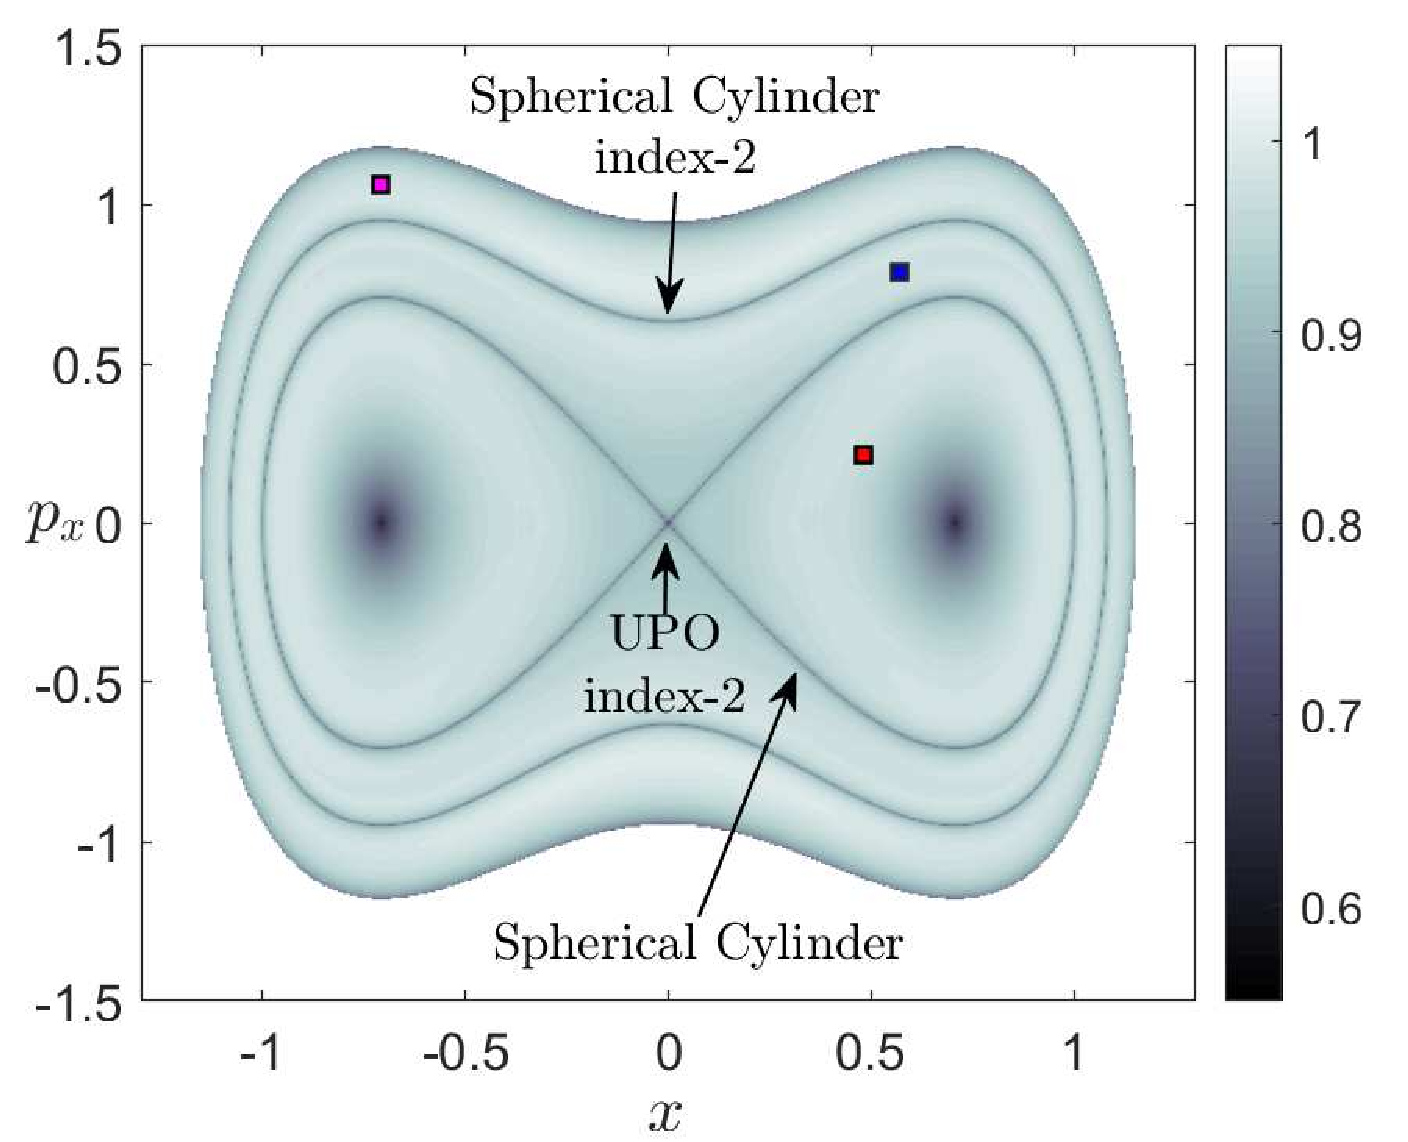
\includegraphics[scale=0.26]{LD_tau_5_y_-1sqrt2_delta_0_H_02}
	\end{center}
	\caption{Example}
	\label{example}
\end{figure}	

One of the biggest challenges when exploring the high-dimensional phase space of a dynamical system is to describe the behavior of ensembles of initial conditions, and to recover from their trajectory evolution the underlying geometrical phase space structures that govern the dynamical mechanisms of the flow. The problem that naturally arises in a   high-dimensional phase space is that the trajectories of ensembles of initial conditions that start nearby might get ``lost'' with respect to each other very quickly, making the use of classical nonlinear dynamics techniques that rely on tracking the location of neighboring trajectories computationally expensive and very difficult to interpret. On the other hand, the method of Lagrangian descriptors provides a revolutionary and radically different approach that resolves this issue, as it focuses on integrating a positive scalar function along the trajectory of any initial condition of the system instead of tracking their phase space location. This is probably one of the key ideas behind the success of this technique, since the phase space geometry is encoded in the initial conditions themselves.

Consider a dynamical system with general time-dependence in the form:
\begin{equation}
\dfrac{d\mathbf{x}}{dt} = \mathbf{v}(\mathbf{x},t) \;,\quad \mathbf{x} \in \mathbb{R}^{n} \;,\; t \in \mathbb{R} \;,
\label{gtp_dynSys}
\end{equation}
where the vector field $\mathbf{v}(\mathbf{x},t) \in C^{r}  (r \geq 1)$ in $\mathbf{x}$ and continuous in time. In order to explore the phase space structures of the dynamical system given by Hamilton's equations in Eq. \eqref{ham_eqs}, we have used in this work the $p$-norm definition of Lagrangian descriptors introduced in \cite{lopesino2017} with $p = 1/2$. Given an initial condition $\mathbf{x}_0$ at time $t_0$, take a fixed integration time $\tau > 0$ and $p \in (0,1]$. The method is defined as follows:
\begin{equation}
M_p(\mathbf{x}_{0},t_0,\tau) = \int^{t_0+\tau}_{t_0-\tau} \, \sum_{i=1}^{n} |v_{i}(\mathbf{x}(t;\mathbf{x}_0),t)|^p \; dt = M_p^{(b)}(\mathbf{x}_{0},t_0,\tau) + M_p^{(f)}(\mathbf{x}_{0},t_0,\tau) \;,
\label{Mp_function}
\end{equation}
where $M_p^{(b)}$ and $M_p^{(f)}$ represent, respectively, backward and forward integration of the initial condition, that is:
\begin{equation}
M_p^{(b)}(\mathbf{x}_{0},t_0,\tau) = \int^{t_0}_{t_0-\tau} \sum_{i=1}^{n} |v_{i}(\mathbf{x}(t;\mathbf{x}_0),t)|^p \; dt \quad,\quad M_p^{(f)}(\mathbf{x}_{0},t_0,\tau) = \int^{t_0+\tau}_{t_0} \sum_{i=1}^{n} |v_{i}(\mathbf{x}(t;\mathbf{x}_0),t)|^p \; dt
\end{equation}
It is important to highlight that with this definition of LDs one can mathematically prove in Hamiltonian systems that NHIMs and their stable and unstable manifolds are detected as singularities of the $M_p$ scalar field, that is, points at which the function is non-differentiable and thus its gradient takes very large values \cite{lopesino2017,demian2017,naik2019a}. Moreover, in this context it has also been shown that:
\begin{equation}
\mathcal{W}^u(\mathbf{x}_{0},t_0) = \textrm{argmin } M_p^{(b)}(\mathbf{x}_{0},t_0,\tau) \quad,\quad \mathcal{W}^s(\mathbf{x}_{0},t_0) = \textrm{argmin } M_p^{(f)}(\mathbf{x}_{0},t_0,\tau)
\label{min_LD_manifolds}
\end{equation}
where $\mathcal{W}^u$ and $\mathcal{W}^s$ are, respectively, the unstable and stable manifolds calculated at time $t_0$ and $\textrm{argmin}(\cdot)$ denotes the phase space coordinates $\mathbf{x}_0$ that minimize the function $M_p$. In addition, NHIMs at time $t_0$ can be calculated as the intersection of the stable and unstable manifolds:
\begin{equation}
\mathcal{N}(\mathbf{x}_{0},t_0) = \mathcal{W}^u(\mathbf{x}_{0},t_0) \cap \mathcal{W}^s(\mathbf{x}_{0},t_0) = \textrm{argmin} M_p(\mathbf{x}_{0},t_0,\tau)
\label{min_NHIM_LD}
\end{equation}
It is important to point out here that the phase space location of the stable and unstable manifolds can be thus obtained in two ways. First, we can extract them as ridges of the scalar function $||\nabla M_p||$ since manifolds are located at points where the function $M_p$ is non-differentiable. Once the manifolds are known, one can compute the NHIM at their intersection by means of a root search algorithm. The second method to recover the manifolds and their associated NHIM is by minimizing the function $M_p$ using a search optimization algorithm. This second procedure and some interesting variations are described in \cite{feldmaier2019}.

As we have mentioned before, NHIMs and their associated stable and unstable manifolds play a crucial role for the analysis of transition dynamics across index-1 saddles that separate two neighboring wells of a PES. This situation is representative for example in chemical isomerization problems, where two wells corresponding to different stable configurations of a given molecule are separated by an energy barrier that the system has to cross in order to undergo an isomerization reaction. In this context, several numerical studies have been carried out recently by means of Lagrangian descriptors to analyze escaping dynamics on open PESs \cite{demian2017,naik2019b,GG2019}. 

At this point, it becomes clear from our discussion that the development of nonlinear techniques that have the capability of unveiling the high-dimensional phase space structures that characterize reaction mechanisms is of paramount importance. The methodology offered by LDs in this respect has been shown to have many advantages. For instance, it is straightforward to implement and computationally inexpensive when applied to systems with two or three DoF. But probably the most important feature of this tool is that it allows to produce a complete and detailed geometrical \textit{phase space tomography} in high dimensions by means of using low-dimensional phase space probes to extract the intersections of the phase space invariant manifolds with these slices \cite{demian2017,naik2019a,naik2019b,GG2019}. 

To finish this section we will illustrate how LDs can be used to detect the geometrical phase space structures, that is, the NHIMs and their stable and unstable invariant manifolds that characterize reaction dynamics between different wells of a PES separated by index-1 saddles. In particular, we will focus on the extraction of the phase space structures for the Hamiltonian system given in Eq. \eqref{ham_eqs} using the model parameters $\alpha = 1$ and considering the symmetric PES, that is $\delta = 0$. We will analyze the phase space structures for the system with energy $H = -0.2$ in the following Poincar\'e surface of section (SOS):
\begin{equation}
\mathcal{P}^{+}_{x,p_x} = \lbrace (x,y,p_x,p_y) \in \mathbb{R}^4 \;|\; y = -1/\sqrt{2} \; ,\; p_y > 0 \rbrace \;.
\label{psos_ld}
\end{equation}
In this case, the energy of the system is below that of the inoemex-2 saddle at the origin but above the energies of the four index-1 saddles surrounding it and connecting the four wells of the PES. Therefore, transport can take place between wells through the phase space bottlenecks that are open in the neighborhood region of the index-1 saddles. The transport mechanism in phase space between different wells is mediated by the stable and unstable manifolds (spherical cylinders) of the unstable periodic orbits (UPOs) corresponding to each index-1 saddle. These geometrical structures act as a 'reactive highway' allowing the system to transit from well to well which would correspond to a given molecule undergoing an isomerization reaction. Suppose that a given molecule starts as an isomer that can be identified with the lower-left well of the PES. The question is: Is it possible to determine the initial conditions of the state of the molecule for which it will transform  into an isomer associated to an adjacent well (sequential isomerization)? The answer to this question is 'yes' and the method of Lagrangian descriptors provides us with the key to unveil the phase space transport routes of this problem. 
Notice that since the chosen energy is below that of the index-2 saddle, the region in the neighborhood of the index-2 saddle is forbidden and thus the system cannot exhibit concerted isomerization, that is, transit from the lower-left well to the upper-right well across the index-2 saddle of the PES. When the system is uncoupled or the coupling is very small, the stable and unstable manifolds of the UPOs of the index-1 saddles of the PES do not give rise to heteroclinic intersections, so that the dynamics of the system remains trapped in the lower-left well or it can exhibit sequential isomerization to the lower-right or upper-left wells. On the other hand, if the DoF of the system are strongly coupled, heteroclinic connections arise between the manifolds of the UPOs of the different index-1 saddles of the PES and the system also admits sequential isomerization from the lower-left to the upper-right well. 

We start our explanation on how to use the method of Lagrangian descriptors by computing it on the Poincar\'e SOS in Eq. \eqref{psos_ld} for the uncoupled system, i.e. $\beta = 0$, using a small integration time $\tau = 5$. Once we have fixed the phase space slice where we want to calculate LDs, we select a grid of initial conditions and, after discarding those that are energetically unfeasible, we integrate the remaining conditions both forward and backward in time, and compute LDs using the definition in Eq. \eqref{Mp_function} with $p = 1/2$. The result is that if we plot the LDs values obtained from the forward/backward integration, the scalar field will reveal the stable/unstable manifolds in the SOS under consideration. Moreover, if we plot the combined sum of forward and backward integration, the method highlights both stable and unstable manifolds simultaneously. This is shown in Fig. \ref{fig:LD_tau5}, where the values of LDs for forward/backward integration is displayed in panel A)/B) and the combination of both is depicted in C). We can clearly see that the manifolds are detected at points where the LD scalar function is non-differentiable. To demonstrate this mathematical property, we represent in Fig. \ref{fig:LD_tau5_maniDetect} the values taken by the LD function along the line $p_x = 0.2$. Notice the jumps in the values of the function, which indicate non-differentiability by means of very large gradient values. Therefore, we can directly extract the invariant stable and unstable manifolds in the Poincar\'e SOS from the gradient, that is, using $||\nabla \mathcal{M}_p||$. This is illustrated in Fig. \ref{fig:LD_mani_extract}  where different values for the integration time have been used to compute LDs, in particular $\tau = 5$ for the uncoupled system, that is $\beta = 0$, and $\tau = 6$, $\tau = 8$ for the coupled system with $\beta = 0.3$. Observe in Fig. \ref{fig:LD_mani_extract}A)-B) that for the uncoupled system, the spherical cylinders of the UPOs of the left and right index-1 saddles do not intersect with the manifolds of the UPO of the bottom index-1 saddle. Moreover, since the system is uncoupled the stable and unstable manifolds for a given UPO coincide. All this shows that if an initial condition starts at the lower-left well of the PES, it can only transit to the lower-right  (upper-left) well if located inside the spherical cylinders of the UPO of the bottom (left) index-1. Once the DoF of the system are coupled, the stable and unstable manifolds of any UPO break apart and, if the coupling is strong enough, they can give rise to homoclinic and heteroclinic connections. The lobes formed by the intricate tangle of the manifolds, in particular, those formed by the manifolds of the UPO of the bottom index-1 with those of the UPOs of the left and right index-1 saddles will have the dynamical effect of allowing an initial condition that starts on the lower-left well of the PES reach, by means of sequential isomerization, the upper-right well. We illustrate in Fig. \ref{fig:LD_mani_extract}C)-F) how the method of Lagrangian descriptors has the capability of unveiling the lobe structure which is crucial for the understanding of the complex dynamical evolution of the system.

It is important to note here the crucial role that the integration time $\tau$ plays when it comes to revealing the invariant manifolds in phase space. As shown in Fig. \ref{fig:LD_mani_extract}, when we increase the value for the integration time, richer and more complex details of the underlying geometrical template of phase space structures is unveiled. This behavior is expected, since an increase of the integration time would imply incorporating more information about the past and future dynamical history of particle trajectories in the computation of LDs. This means that $\tau$ is intimately related to the time scales of the dynamical phenomena that take place in the model under consideration and thus, it is a parameter that is problem-dependent. Consequently, there is no general ``golden'' rule for selecting its value for exploring phase space, and thus it is usually selected from the information obtained by performing several numerical experiments. One needs to always bare in mind that there is a compromise between the complexity of the structures that one would like to reveal to explain a certain dynamical mechanism, and the interpretation of the intricate manifolds displayed in the LD scalar output. 




As a final remark, there is a key point that needs to be highlighted with regard to the application of LDs and that demonstrates the real potential of this tool with respect to other classical nonlinear dynamics techniques. We have seen that one can extract the stable and unstable manifolds from the gradient of the $M_p$ function and therefore obtain \textit{all} the manifolds coming from \textit{any} NHIM in phase space \textit{at the same time}. This is of course a tremendous advantage in comparison to the classical approach of computing stable and unstable manifolds that relies on locating first the NHIMs in phase space individually, and for every NHIM globalize the manifolds separately, for which a knowledge of the eigendirections is crucial. Consequently, the application of LDs offers the capability of recovering \textit{all} the relevant phase space structures in one \textit{shot} without having to study the local dynamics about equilibrium points of the dynamical system.









\bibliography{LDs}

\end{document}

